\documentclass[12pt]{article}

\usepackage{epsfig,array,amsmath,fancybox,epic}

\usepackage[latin1]{inputenc}

\voffset=-2cm
\hoffset=-1cm

\setlength{\textheight}{25cm}
\setlength{\textwidth}{16cm}
\setlength{\parindent}{0cm}

%-------------------------------------------------------------------------
\setlength{\fboxsep}{3mm}
%-------------------------------------------------------------------------

\begin{document}

\begin{LARGE}
\begin{bf}
\begin{center}
Biblioth\`eque de gestion d'images

\end{center}
\end{bf}
\end{LARGE}

\section{Introduction}

Cette biblioth\`eque de gestion d'images permet, assez simplement, de
cr\'eer des images (en niveaux de gris ou en couleurs), de les
manipuler et de les afficher.\\
De plus, 3 formats d'images sont pris
en charge pour la lecture ou l'\'ecriture de fichiers image~:
{\tt .ras} (Sun Rasterfile), {\tt .ppm} et {\tt .pgm}~.

\section{Les classes {\tt Image} et {\tt ImageRVB}}

Cette section d\'ecrit bri\`evement les classes permettant de
manipuler des images~:
\begin{itemize}
\item[-] {\tt class Image} ; pour la manipulation d'images
en niveaux de gris sur 1 plan o\`u chaque pixel est
cod\'e sur 1 octet ({\tt typedef unsigned char octet;}).
\item[-] {\tt class ImageRVB} ; pour la manipulation d'images
couleurs sur 3 plans (3 objets de la classe {\tt Image}).
\end{itemize}

\begin{figure}[hbtp]
\begin{center}
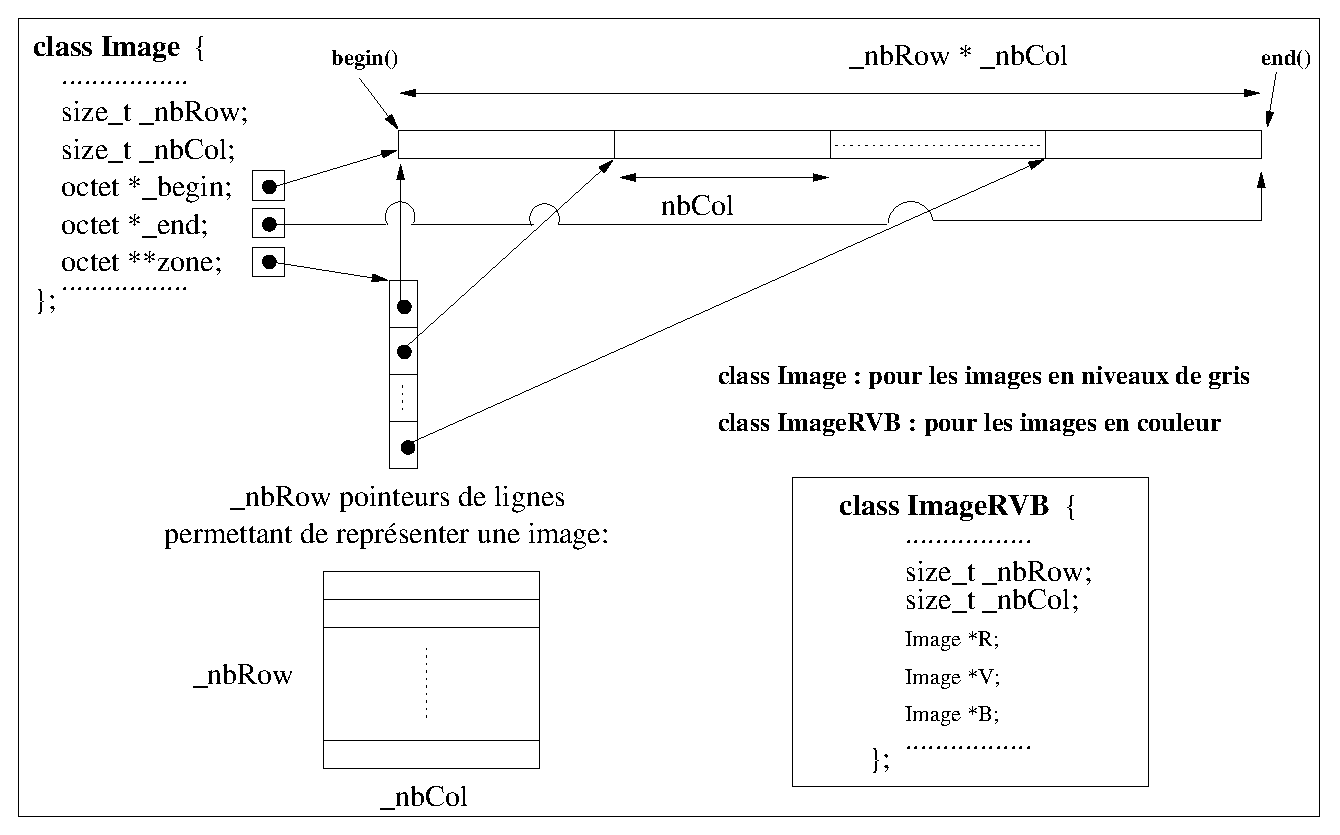
\includegraphics[width=15.5cm]{fig/classImage}
\end{center}
\caption{Description des structures internes des deux classes
{\tt Image} et {\tt ImageRVB}.}
\end{figure}

\newpage

\section{Interface publique de la classe {\tt Image}}

\vspace{-0.1cm}
\begin{footnotesize}
\begin{verbatim}
class Image {
              friend ostream& operator<<(ostream& os, const Image& anImage);
\end{verbatim}
\end{footnotesize}
\vspace{-0.4cm}
\begin{footnotesize}
\begin{verbatim}
  public:
\end{verbatim}
\vspace{-0.3cm}
\begin{verbatim}
    // Allocateurs/Desallocateurs
\end{verbatim}
\vspace{-0.2cm}
\begin{verbatim}
           Image(size_t nbRow=512, size_t nbCol=512);
           Image(const char* fileName);
           Image(const Image& anImage);
           Image(const ImageRVB& anImageRVB);            // Cousin... I_NB <- I_RVB
           Image& operator=(const Image& anImage);       // Affectation
           Image& operator=(const ImageRVB& anImageRVB); // Affectation : I_NB <- I_RVB
  virtual ~Image(void);

           void  setImageSize(size_t nbRow, size_t nbCol);

           void  loadImage(const char* fileName);
           void  saveImage(const char* fileName);

    // Operateurs
\end{verbatim}
\vspace{-0.3cm}
\begin{verbatim}
           Image& operator+=(const Image& anImage);
    friend Image  operator+ (const Image& anImage1,const Image& anImage2);
           Image& operator-=(const Image& anImage);
    friend Image  operator- (const Image& anImage1,const Image& anImage2);

    // Comparaisons
\end{verbatim}
\vspace{-0.3cm}
\begin{verbatim}
  friend   bool operator==(const Image& anImage1, const Image& anImage2);
  friend   bool operator!=(const Image& anImage1, const Image& anImage2);

    // Inspecteurs
\end{verbatim}
\vspace{-0.3cm}
\begin{verbatim}
           size_t  getNbRow(void) const;
           size_t  getNbCol(void) const;

     const octet*  begin(void) const; // Un pointeur sur le DEBUT
           octet*  begin(void);       // de la zone image
     const octet*  end(void) const;   // Un pointeur sur la FIN
           octet*  end(void);         // de la zone image

    // Modificateurs/Inspecteurs
\end{verbatim}
\vspace{-0.3cm}
\begin{verbatim}
           void  writePix(size_t row, size_t col, octet val);
           void  readPix(size_t row, size_t col, octet& val) const;
           octet readPix(size_t row, size_t col) const;

           const octet* operator[] (size_t row) const;    // Pour autoriser
                 octet* operator[] (size_t row);          // anImage[row][col]

           octet  operator() (size_t row, size_t col) const; // Pour autoriser
           octet& operator() (size_t row, size_t col);       // anImage(row,col)

           void  setImage(octet val); // Tous les pixels initialises a val
           void  lineImage(int X1,int Y1, int X2,int Y2,octet val); // Ligne (x1,y1)-(x2,y2)

  protected:
\end{verbatim}
\vspace{-0.3cm}
\begin{verbatim}
  //  display a appeler dans une classe derivee (methode appelee dans operator<<)
   virtual void display(ostream& os) const;
\end{verbatim}
\begin{verbatim}
  //  isEqualTo a appeler dans une classe derivee (methode appelee dans operator==)
   virtual bool isEqualTo(const Image& anImage) const;
};
\end{verbatim}
\end{footnotesize}

\section{Interface publique de la classe {\tt ImageRVB}}

\vspace{-0.3cm}
\begin{footnotesize}
\begin{verbatim}
class ImageRVB {
                 friend ostream& operator<<(ostream& os, const ImageRVB& anImageRVB);
  public:
\end{verbatim}
\vspace{-0.3cm}
\begin{verbatim}
    // Allocateurs/Desallocateurs
\end{verbatim}
\vspace{-0.2cm}
\begin{verbatim}
           ImageRVB(size_t nbRow=512, size_t nbCol=512);
           ImageRVB(const char* fileName);
           ImageRVB(const ImageRVB& anImageRVB);
           ImageRVB(const Image& anImage);                  // Cousin... I_RVB <- I_NB
           ImageRVB& operator=(const ImageRVB& anImageRVB); // Affectation
           ImageRVB& operator=(const Image& anImage);       // Affectation: I_RVB <- I_NB
  virtual ~ImageRVB(void);

           void  setImageSize(size_t nbRow, size_t nbCol);

           void  loadImage(const char* fileName);
           void  saveImage(const char* fileName);
\end{verbatim}
\vspace{-0.2cm}
\begin{verbatim}
    // Operateurs
\end{verbatim}
\vspace{-0.2cm}
\begin{verbatim}
           ImageRVB& operator+=(const ImageRVB& anImageRVB);
    friend ImageRVB  operator+ (const ImageRVB& anImageRVB1, const ImageRVB& anImageRVB2);
           ImageRVB& operator-=(const ImageRVB& anImageRVB);
    friend ImageRVB  operator- (const ImageRVB& anImageRVB1, const ImageRVB& anImageRVB2);
\end{verbatim}
\vspace{-0.2cm}
\begin{verbatim}
    // Comparaisons
\end{verbatim}
\vspace{-0.2cm}
\begin{verbatim}
  friend   bool operator==(const ImageRVB& anImageRVB1, const ImageRVB& anImageRVB2);
  friend   bool operator!=(const ImageRVB& anImageRVB1, const ImageRVB& anImageRVB2); 

    // Inspecteurs
\end{verbatim}
\vspace{-0.2cm}
\begin{verbatim}
           size_t  getNbRow(void) const;
           size_t  getNbCol(void) const;

     const Image&  getR(void) const;          // Pour obtenir
           Image&  getR(void);                // le plan R

     const Image&  getV(void) const;          // Pour obtenir
           Image&  getV(void);                // le plan V

     const Image&  getB(void) const;          // Pour obtenir
           Image&  getB(void);                // le plan B
\end{verbatim}
\vspace{-0.2cm}
\begin{verbatim}
    // Modificateurs/Inspecteurs
\end{verbatim}
\vspace{-0.2cm}
\begin{verbatim}
           void  writePix(size_t row, size_t col, octet valR, octet valV, octet valB);
           void  readPix(size_t row, size_t col, octet& valR, octet& valV, octet& valB) const;

           void  setImage(octet valR, octet valV, octet valB); // Tous les pixels initialises
                                                               // a valR, valV et valB

           void  lineImage(int X1,int Y1, int X2,int Y2, octet valR, // Ligne (x1,y1)-(x2,y2)
                                                         octet valV,
                                                         octet valB);
\end{verbatim}
\vspace{-0.2cm}
\begin{verbatim}
  protected:
\end{verbatim}
\vspace{-0.2cm}
\begin{verbatim}
  //  display a appeler dans une classe derivee (methode appelee dans operator<<)
   virtual void display(ostream& os) const;

  //  isEqualTo a appeler dans une classe derivee (methode appelee dans operator==)
   virtual bool isEqualTo(const ImageRVB& anImageRVB) const;
};
\end{verbatim}
\end{footnotesize}

\section{M\'ethodes d'acc\`es aux images de la classe {\tt Image}}

Afin d'illustrer les diff\'erentes possibilit\'es d'acc\`es \`a
une image en niveaux de gris, nous prenons l'exemple d'une fonction
{\tt raz} permettant de mettre \`a {\tt 0} tous les pixels d'une image.

\vspace{-0.2cm}
\subsection{Avec des [~][~]}

\begin{footnotesize}
\begin{verbatim}
void raz(Image& out)
{
 int nbRow = out.getNbRow(), nbCol = out.getNbCol();
 for(int l=0;l<nbRow;l++)
 {
  for(int c=0;c<nbCol;c++)
  {
   out[l][c] = 0;       // Pas de test de validite de l et c ... plus rapide
  }                     //                                   ... moins fiable
 }
}
\end{verbatim}
\end{footnotesize}

\vspace{-0.3cm}
\subsection{Avec des (~,~)}

\begin{footnotesize}
\begin{verbatim}
void raz(Image& out)
{
 int nbRow = out.getNbRow(), nbCol = out.getNbCol();
 for(int l=0;l<nbRow;l++)
 {
  for(int c=0;c<nbCol;c++)
  {
   out(l,c) = 0;              // Test de validite de l et c ... moins rapide
  }                           //                            ... plus fiable
 }
}
\end{verbatim}
\end{footnotesize}

\vspace{-0.3cm}
\subsection{Avec un acc\`es via un pointeur (parcours s\'equentiel)}

\begin{footnotesize}
\begin{verbatim}
void raz(Image& out)
{
 for(octet* ptrOut = out.begin() ; ptrOut < out.end() ; ptrOut++)
 {
  *ptrOut = 0;
 }
}
\end{verbatim}
\end{footnotesize}

\vspace{-0.3cm}
\subsection{Avec un appel de m\`ethode {\tt readPix} ou {\tt writePix}}

\begin{footnotesize}
\begin{verbatim}
void raz(Image& out)
{
 int nbRow = out.getNbRow(), nbCol = out.getNbCol();
 for(int l=0;l<nbRow;l++)
 {
  for(int c=0;c<nbCol;c++)
  {
   out.writePix(l,c,0);       //  Test de validite de l et c ... moins rapide
  }                           //                             ... plus fiable
 }
}
\end{verbatim}
\end{footnotesize}

\section{M\'ethodes d'acc\`es aux images de la classe {\tt ImageRVB}}

Afin d'illustrer les diff\'erentes possibilit\'es d'acc\`es \`a
une image en couleur, nous prenons l'exemple d'une fonction {\tt raz}
permettant de mettre \`a {\tt 0} tous les pixels d'une image.

\subsection{Avec un appel de m\'ethode {\tt readPix} ou {\tt writePix}}

\begin{footnotesize}
\begin{verbatim}
void raz(ImageRVB& out)
{
 int nbRow = out.getNbRow(), nbCol = out.getNbCol();
 for(int l=0;l<nbRow;l++)
 {
  for(int c=0;c<nbCol;c++)
  {
   out.writePix(l,c,0,0,0);   //  Test de validite de l et c
  }
 }
}
\end{verbatim}
\end{footnotesize}

\subsection{En obtenant des r\'ef\'erences sur les diff\'erents
plans {\tt Image}}

\begin{footnotesize}
\begin{verbatim}
void raz(ImageRVB& out)
{
 Image& R = out.getR();
 Image& V = out.getV();
 Image& B = out.getB();

 raz(R);  // Appels a la methode raz pour chaque plan, methode
 raz(V);  // decrite lors de la section precedente... sur les
 raz(B);  // objet de la classe Image
}
\end{verbatim}
\end{footnotesize}

\section{Redimensionnement d'une image}

Il peut parfois \^etre n\'ecessaire de redimensionner
une image avant un traitement avec la m\'ethode
{\tt setImageSize} de la classe {\tt Image} ou de la
classe {\tt ImageRVB}.
Ainsi, si l'on consid\`ere l'exemple suivant~:

\begin{footnotesize}
\begin{verbatim}
void seuillage(const Image& in, Image& out, octet seuil)
{
 int nbRow = in.getNbRow(), nbCol = in.getNbCol();

 out.setImageSize(nbRow,nbCol);  // Redimensionnement, ... au cas ou

 for(int l=0;l<nbRow;l++)
 {
  for(int c=0;c<nbCol;c++)
  {
   out[l][c] = (in[l][c] > seuil) ? 0 : 255;   // Pas de test de validite de l et c
  }
 }
}
\end{verbatim}
\end{footnotesize}

un redimensionnement de l'image de sortie sera ainsi effectu\'e.
Remarque~: il n'y a r\'eallocation de la zone d\'edi\'ee \`a l'image
que si les dimensions n'\'etaient pas celles d\'esir\'ees.

\section{Passage d'une {\tt Image} \`a une {\tt ImageRVB} et inversement}

Afin de facilier la transformation d'une {\tt ImageRVB} en une {\tt Image},
il existe dans la classe {\tt Image} un constructeur par cousinage et
un op\'erateur d'affectation permettant de faire la conversion d'une image
cod\'ee sur 3 plans en une image cod\'ee sur 1 plan~:

\begin{footnotesize}
\begin{verbatim}
 Image(const ImageRVB& anImageRVB);            // Cousin... I_NB <- I_RVB
 Image& operator=(const ImageRVB& anImageRVB); // Affectation : I_NB <- I_RVB
\end{verbatim}
\end{footnotesize}

Dans la classe {\tt ImageRVB}, il existe \'egalement la possibilit\'e
de convertir une {\tt Image} en une {\tt ImageRVB}~:

\begin{footnotesize}
\begin{verbatim}
 ImageRVB(const Image& anImage);            // Cousin... I_RVB <- I_NB
 ImageRVB& operator=(const Image& anImage); // Affectation : I_RVB <- I_NB
\end{verbatim}
\end{footnotesize}



\ifnum 1 = 0
Dans la classe {\tt Image}, il y a une m\'ethode
permettant de transformer une {\tt ImageRVB} en une {\tt Image}~:

\begin{footnotesize}
\begin{verbatim}
void Image::ImageRVB2Image(const ImageRVB& anImageRVB); // I_RVB -> I_NB
\end{verbatim}
\end{footnotesize}

Dans la classe {\tt ImageRVB}, il y a une m\'ethode
permettant de transformer une {\tt Image} en une {\tt ImageRVB}~:

\begin{footnotesize}
\begin{verbatim}
void ImageRVB::Image2ImageRVB(const Image& anImage); // I_NB -> I_RVB
\end{verbatim}
\end{footnotesize}

\fi

\section{Affichage d'une image ({\tt Image} ou {\tt ImageRVB})}

Afin d'afficher une image, if faut d\'eclarer un objet de
type {\tt XAffichage} en indiquant les dimensions de la
fen\^etre d'affichage.

Ensuite, sur cet objet, il faut appeler~:
\begin{itemize}
\item[-] la m\'ethode {\tt Afficher} en passant l'image
({\tt Image} ou {\tt ImageRVB}) \`a afficher.
\item[-] Puis, la m\'ethode {\tt XEvenement} (toujours
en passant l'image).
Cette m\'ethode retourne un \'eventuel caract\`ere
ayant \'et\'e entr\'e par l'utilisateur.
\end{itemize}

Ainsi, le programme type d'affichage d'une image
est le suivant. 

\begin{scriptsize}
\begin{verbatim}
       // g++ ex.cpp -I../LibImages/include -L/usr/X11R6/lib -lX11 -L../LibImages/lib -lImages -o ex 
\end{verbatim}
\end{scriptsize}

\begin{footnotesize}
\begin{verbatim}
#include <iostream>             // Fichier ex.cpp

using namespace std;

#include "LibImages.h"

int main(void)
{
 ImageRVB im("../Images/Lena/lena24FullColor.ras");

 XAffichage *Fim = new XAffichage(im.getNbRow(),im.getNbCol());
 Fim->setLabel("lena24FullColor.ras");

 while (1)
 {
  char cim;

  Fim->Afficher(im);
  cim=Fim->XEvenement(im);
  cim = tolower(cim);

  if (cim=='q')  break;
 }

 delete(Fim);

 return 0;
}
\end{verbatim}
\end{footnotesize}

\section{Affichage d'une image ({\tt Image} ou {\tt ImageRVB}) avec gestion
de la souris}

\begin{scriptsize}
\begin{verbatim}
 // g++ exCurseur.cpp -I../LibImages/include -L/usr/X11R6/lib -lX11 -L../LibImages/lib -lImages -o exCurseur 
\end{verbatim}
\end{scriptsize}
\begin{footnotesize}
\begin{verbatim}
#include <iostream>             // Fichier exCurseur.cpp

using namespace std;

#include "LibImages.h"

int main(void)
{
 ImageRVB im("../Images/Lena/lena24FullColor.ras");

 XAffichage *Fim = new XAffichage(im.getNbRow(),im.getNbCol());
 Fim->setLabel("lena24FullColor.ras");

 while (1)
 {                                 /***************************************/
  XAffichageEvent event;           /* Dans un XAffichageEvent, il y a:    */
                                   /*                                     */
  /* typedef                    */ /* 1) Recuperation caractere appuye:   */
  /*    struct {                */ /*                                     */
  /*      char key;             */ /* char key (le caractere appuye ou    */
  /*      int  button;          */ /*           -1 si aucun caractere)    */
  /*      int  row;             */ /* key...aussi le retour de XEvenement */
  /*      int  col;             */ /*                                     */
  /*      bool onButtonPress;   */ /* 2) Gestion souris:                  */
  /*      bool onButtonRelease; */ /*                                     */
  /*      bool onButtonMotion;  */ /* int button (1,2 ou 3 si evt souris  */
  /*    } XAffichageEvent;      */ /*             -1 si aucun evt souris) */
                                   /* Si button!= -1 :                    */
  char cim;                        /* . int row,int col(coord y,x souris) */
                                   /*     (row,col)=(-1,-1) si en dehors  */
  Fim->Afficher(im);               /* . bool onButtonPress  (true,false), */
  cim=Fim->XEvenement(im,&event);  /* . bool onButtonRelease(true,false), */
  cim = tolower(cim);              /* . bool onButtonMotion (true,false). */
  if (event.button>0)              /***************************************/
  {
   if (event.onButtonPress)   { cout << "  Press";   }
   else
   if (event.onButtonRelease) { cout << "Release"; }
   else
   if (event.onButtonMotion)  { cout << " Motion"; }
   else { cout << "???????"; }

   cout << "(" << event.button << "):";
   cout<<"("<<event.button<<"):"<<" row: "<<event.row<<" col: "<< event.col;
   cout << endl;
  }
\end{verbatim}
\begin{verbatim}
  if (cim=='q')  break;
 }
\end{verbatim}
\begin{verbatim}
 delete(Fim);
\end{verbatim}
\begin{verbatim}
 return 0;
}
\end{verbatim}
\end{footnotesize}

\section{Affichage avec un visalisateur externe}

La fonction
\begin{center}
{\tt void displayImage(const char *nomFichier, char *visualiseur = "xv");}
\end{center}
fonction d\'ecrite dans le fichier {\tt LibImages/src/ESImages.cpp},
permet d'afficher le contenu d'un fichier image \`a l'aide d'un
visualisateur externe.

Par d\'efaut, le visualisateur externe utilis\'e est
{\tt xv}.

\vspace{0.3cm}

Exemples d'utilisation~:

\begin{footnotesize}
\begin{verbatim}
displayImage("../Images/Lena/lena24FullColor.ras");        // Affichage avec xv

displayImage("../Images/Lena/lena24FullColor.ras","gimp"); // Affichage avec gimp
\end{verbatim}
\end{footnotesize}

\section{Formats image pris en charge lors
du chargement ou de la sauvegarde d'une image}

\subsection{Lors du chargement}

Lors du chargement d'une image ({\tt Image} ou {\tt ImageRVB})
avec le constructeur ou la m\'ethode {\tt loadImage},
les formats pris en charge sont {\tt .ras}, {\tt .ppm} et {\tt .pgm}~.

La d\'etection du format se fait via l'extension du
fichier~:
\begin{itemize}
\item[-] {\tt .ras} ; format de Sun : rasterfile
\item[-] {\tt .ppm} ; format PPM : Portable PixMap (binaire ou ascii)
\item[-] {\tt .pgm} ; format PGM : Portable GreyMap (binaire ou ascii)
\end{itemize}

\subsection{Lors de la sauvegarde}

Lors de la sauvegarde d'une image ({\tt Image} ou {\tt ImageRVB})
avec la m\'ethode {\tt saveImage},

les formats pris en charge sont {\tt .ras}, {\tt .ppm} et {\tt .pgm}~.

La d\'etection du format se fait via l'extension du
fichier~:
\begin{itemize}
\item[-] {\tt .ras} ; format de Sun : rasterfile
\item[-] {\tt .ppm} ; format PPM (Portable PixMap) binaire
\item[-] {\tt .ascii.ppm} ; format PPM (Portable PixMap) acsii
\item[-] {\tt .pgm} ; format PGM (Portable GreyMap) binaire
\item[-] {\tt .ascii.pgm} ; format PGM (Portable GreyMap) acsii
\end{itemize}

\newpage

\section{A savoir}

Il est possible:
\begin{itemize}
\item de tester l'\'egalit\'e ou l'in\'egalit\'e entre deux images

$\Longrightarrow$ {\tt operator==} et {\tt operator!=}

\item d'affecter une image dans une autre

$\Longrightarrow$ {\tt operator=}

\item de calculer la somme de deux images

$\Longrightarrow$ {\tt operator+=} et {\tt operator+}

\item de calculer la diff\'erence de deux images

$\Longrightarrow$ {\tt operator-=} et {\tt operator-}
\end{itemize}

Remarque: ces op\'erateurs existent pour la classe {\tt Image}
et pour la classe {\tt ImageRVB}

\section{Installation}

\begin{figure}[hbtp]
\begin{center}
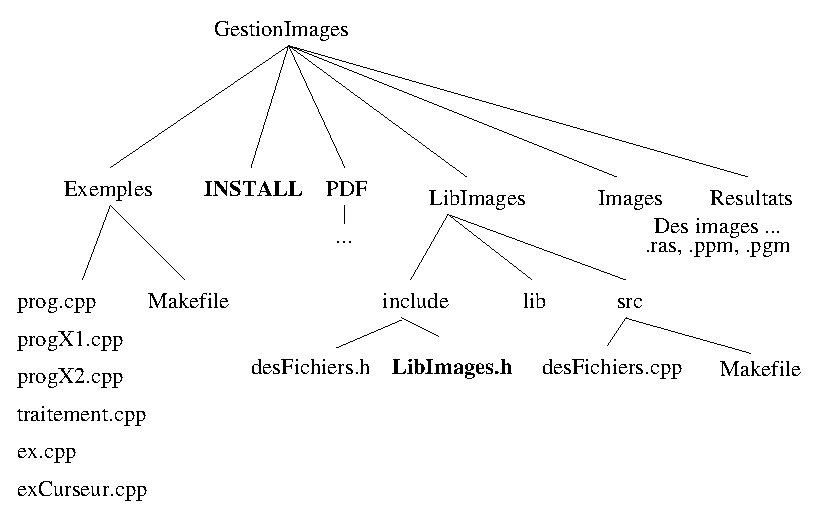
\includegraphics[width=13.5cm]{fig/arbo}
\caption{Description de l'arborescence de la biblioth\`eque}
\end{center}
\end{figure}

Aller dans le r\'epertoire {\tt LibImages/src}
et faire {\tt \$ make}

Une biblioth\`eque {\tt libImages.a} est alors plac\'ee dans le r\'epertoire
{\tt LibImages/lib}

Des exemples de programmes sont disponibles dans le r\'epertoire
{\tt Exemples} (un fichier {\tt Makefile} est donn\'e). 

\vspace{0.5cm}
{\bf ... mais on peut faire plus simple !}

\vspace{0.3cm}

En \'etant dans le r\'epertoire {\tt GestionImages}, faire tout
simplement {\tt \$ ./INSTALL}

Il faut ensuite aller dans le r\'epertoire {\tt Exemples}
et faire {\tt \$ make}

\end{document}
